%Plantilla anteproyecto TFG
%Última modificación: 28 de mayo de 2021
\documentclass[12pt,oneside,a4paper]{article}
\usepackage[spanish]{babel}
\usepackage[utf8]{inputenc}
\usepackage{graphicx}
\usepackage{amsmath}
\usepackage{amssymb}
\usepackage{xcolor}
\usepackage{subfigure}
\usepackage{url}
\usepackage{float}
\linespread{1}
\usepackage{multirow}
\usepackage{colortbl}
\usepackage{rotating}
\usepackage[pagebackref=true,breaklinks=true,letterpaper=true,colorlinks=true,linkcolor=black,bookmarks=true]{hyperref}

\usepackage[spanish]{babel}
\usepackage[utf8]{inputenc}

\usepackage{transparent}
\usepackage{eso-pic}
 
\usepackage{blindtext}

\makeindex
\setlength{\parskip}{1\baselineskip}
\parindent 1cm
\sloppy


%Opciones que debes descomentar mientras estemos revisando el anteproyecto
\usepackage{lineno}
\linenumbers


\usepackage[pagebackref=true,breaklinks=true,letterpaper=true,colorlinks,bookmarks=true]{hyperref}


%lista de palabras que Latex no parte bien
\hyphenation{pa-la-bras lis-ta}

\begin{document}
\AddToShipoutPicture{
\put(0,0){
\parbox[b][\paperheight]{\paperwidth}{%
\vfill
\centering
{\transparent{0.1}
\includegraphics[scale=1.5]{figuras/logo-uah.jpg}}%
\vfill
}
}
}

\thispagestyle{empty}

\begin{center}

\begin{large}
UNIVERSIDAD DE ALCALÁ\\
Escuela Politécnica Superior\\
\end{large}
\vspace{4cm}


\begin{Huge}\textbf{\textit{Innovación Tecnológica en la Evaluación Geriátrica: Automatización de Pruebas SPPB mediante Aplicación Móvil y Plataforma Web}}\end{Huge}

\vspace{1cm}


\textbf{ANTEPROYECTO FIN DE GRADO}

\vfill
\hline
Abril - 2024

\end{center}

\begin{flushright}
\textit{Autor - \textbf{F. Javier Redondo García}} \\
\textit{Tutor - \textbf{Sergio Caro Álvaro}} \\
\textit{Cotutora - \textbf{Ana Jiménez Martín}}

\end{flushright}


\newpage
\tableofcontents

\newpage
\section{Introducción}
\hline

El envejecimiento fisiológico eleva la incidencia de enfermedades y éstas repercuten en aspectos funcionales, lo que favorece la incapacidad. Se pretende detectar el decaimiento físico en sus etapas más tempranas para intentar retrasar el estado de fragilidad. Para ello se utiliza el Test de evaluación del desempeño físico \cite{welch2021short} (SPPB) del adulto mayor como ayuda a la valoración geriátrica integral. \\
El Test consiste en la realización de tres pruebas a cada uno de los pacientes. El protocolo de las pruebas es el siguiente: \\
\begin{itemize}
\item Prueba de equilibrio: Se debe aguantar 10 segundos en tres posiciones diferentes (pies juntos, semitándem y tándem), sin ningún tipo de apoyo. \\
\item Prueba de velocidad de la marcha en 4 metros: Se mide el tiempo que tarda el paciente en recorrer 4 metros en línea recta. Se realizan dos pruebas.\\
\item Prueba de levantarse de la silla 5 veces: El paciente debe levantarse de la silla lo más rápido que pueda sin utilizar los brazos. Se mide el tiempo que tarda en hacerlo.
\end{itemize}
Según el desempeño que el paciente haya tenido en las pruebas, se le asignan unos puntos, con los que el profesional sanitario determina la probabilidad de fragilidad.

\section{Planteamiento del problema}
\hline
Cada una de las pruebas tienen unas medidas constantes, y uno de los grandes beneficios del test SPPB es poder realizar las mismas pruebas a lo largo del tiempo, comprobando así si la puntuación (y con esto la probabilidad de fragilidad) aumenta, se mantiene o disminuye. 
A día de hoy estas pruebas se realizan de manera manual, de esta manera se contemplan posibles errores en el registro de los datos, además de la posible subjetividad del personal sanitario.

Por otro lado, al obtener los datos de manera manual, la complejidad de recopilar la información en una base de datos, donde se pueda ver cada paciente y analizar cada prueba a lo largo del tiempo aumenta significativamente. 


\section{Objetivo}
\hline
Se pretende  facilitar, agilizar y mejorar la intervención médica con ayuda tecnológica. El proyecto pretende proporcionar herramientas que eliminen los errores que se pueden cometer al hacer las pruebas de manera manual y que no exijan amplios conocimientos técnicos, ayudando al equipo sanitario a tener un control sobre cada prueba realizada a cada paciente, así como una base de datos donde quede registrada toda la información necesaria.


\section{Metodología}\index{Metodología} \\
\hline
La propuesta se compone de tres tareas fundamentales: 

\subsection{ANÁLISIS Y SELECCIÓN DE LA BASE DE DATOS ADECUADA}
Existen diferentes tipos de bases de datos atendiendo a su estructura y al modelo de datos que utilizan. En este apartado se deberá hacer un análisis de qué tipos de datos vamos a tener y qué estructura es óptima para almacenarlos.

\subsection{DESARROLLO DE APLICACIÓN MOVIL}
Hoy en día está sumamente extendido el uso de Smartphones que tienen conexión a internet, Bluethooth y un alcance de procesamiento muy potente. Con esto se pretende desarrollar una aplicación que conectada con ........................ recoja los datos en crudo y haga todo el procesamiento, convirtiendo los datos en crudo en, finalmente, puntos SPPB. Este dispositivo deberá estar conectado a internet para, una vez terminada la prueba, subir la información a la base de datos, donde quedará registrada y estructurada.

\subsection{DESARROLLO DE SERVIDOR WEB} 
Se pretende desarrollar un servidor Web con una interfaz sencilla, cuyo objetivo sea recopilar la información de la base de datos y representarla para que el personal sanitario pueda hacer el análisis de las pruebas y llevar un control del histórico de sus pacientes. \\

\hline

\begin{figure}[H]
  \centering
  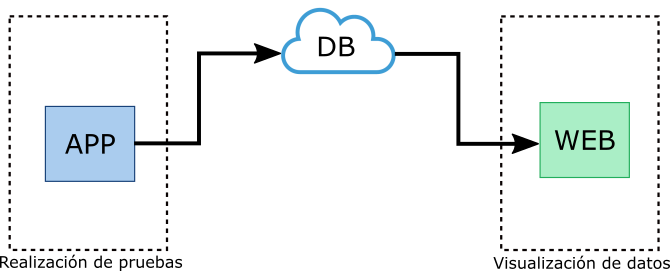
\includegraphics[width=15cm]{anteproyecto/figuras/tfg_diagramabloques_simple.png}
  \caption{Diagrama de bloques del funcionamiento básico del proyecto}
  \label{fig:ejemplo}
\end{figure}

\newpage

\section{Cronograma de actividades}
\hline

La planificación temporal correspondiente a estas fases está definida del siguiente modo: 
\begin{table}[H]
\begin{tabular}{|l|l|c|c|c|c|}
\hline
\rowcolor[HTML]{DAE8FC} 
Fases                        & Actividad                                         & \multicolumn{1}{l|}{\cellcolor[HTML]{DAE8FC}Abril} & \multicolumn{1}{l|}{\cellcolor[HTML]{DAE8FC}Mayo} & \multicolumn{1}{l|}{\cellcolor[HTML]{DAE8FC}Junio} & \multicolumn{1}{l|}{\cellcolor[HTML]{DAE8FC}Julio} \\ \hline
Inicio                       & Análisis del funcionamiento del test SPPB         & X                                                  &                                                   &                                                    &                                                    \\ \hline
                             & Análisis y selección de la base de datos adecuada & X                                                  &                                                   &                                                    &                                                    \\ \cline{2-6} 
                             & Desarrollo de aplicación móvil                    & X                                                  & X                                                 & X                                                  &                                                    \\ \cline{2-6} 
\multirow{-3}{*}{Desarrollo} & Desarrollo de aplicación web                      &                                                    & X                                                 & X                                                  &                                                    \\ \hline
                             & Redacción de la memoria                           &                                                    & X                                                 & X                                                  &                                                    \\ \cline{2-6} 
\multirow{-2}{*}{Final}      & Preparación de la defensa                         &                                                    &                                                   &                                                    & X                                                  \\ \hline
\end{tabular}
\caption{Planificación temporal}
\end{table}


\section{Medios disponibles}
\hline

    \subsection{Aplicación móvil} Se hará uso de un teléfono móvil con sistema operativo Android versión 11 o superior. Este teléfono debe tener acceso a internet para poder comunicarse con la base de datos.
     El desarrollo Android se hará usando el entorno de desarrollo nativo Android Studio \cite{hohensee2014introduccion}. \\

    \subsection{Servidor web} En cuanto a la web, se desarrollará con el lenguaje de programación Typescript, que trabaja sobre JavaScript y que permite añadir características estáticas de tipo, clases y módulos opcionales a JS. \\ 
    Como entorno de desarrollo se utilizará Angular \cite{wilken2018angular}, framework que ofrece un conjunto de herramientas completo y potente, que puede ser ideal para el objetivo del proyecto. \\

    \subsection{Redacción de la memoria} Se utilizará Overleaf, una plataforma online para la edición y compilación de documentos escritos en el sistema de composición de textos \LaTeX \cite{wikibook}\\

    \subsection{General} Se hará uso de un ordenador que tenga instalado el sistema operativo Windows y un mínimo de 8Gb de memoria RAM. Además, para llevar un control de versiones se utilizará el programa GitHub.






%Bibliografía
\section{Referencias}

\bibliography{bibliografia-tfc}
\bibliographystyle{ieeetr}


\end{document}
